\documentclass[aspectratio=169]{beamer}
\usetheme{Madrid}
\usecolortheme{default}

\usepackage{fontspec}
\usepackage{polyglossia}
\setmainlanguage{spanish}
\usepackage{graphicx}
\usepackage{amsmath}
\usepackage{booktabs}
\usepackage{xcolor}

\definecolor{usalred}{RGB}{140,21,21}
\definecolor{usalreddark}{RGB}{80,10,10}
\usecolortheme[named=usalred]{structure}
\setbeamercolor{title}{bg=usalred,fg=white}
\setbeamercolor{frametitle}{bg=usalred,fg=white}
\setbeamercolor{palette primary}{bg=usalred,fg=white}
\setbeamercolor{palette secondary}{bg=usalreddark,fg=white}
\setbeamercolor{palette tertiary}{bg=usalreddark,fg=white}
\setbeamercolor{palette quaternary}{bg=usalred,fg=white}
\setbeamercolor{block title}{bg=usalred,fg=white}
\setbeamercolor{section in toc}{fg=usalred}

\setbeamertemplate{navigation symbols}{}
\setbeamerfont{footnote}{size=\tiny}

\setbeamercolor{footlinebox}{bg=usalreddark,fg=white}
\setbeamertemplate{footline}{
  \leavevmode
  \hbox{%
  \begin{beamercolorbox}[wd=.55\paperwidth,ht=2.6ex,dp=1.2ex,left,leftskip=1em]{footlinebox}
    \usebeamerfont{footline}\tiny Fundamentos e introducción al aprendizaje automático --- Cap. 2
  \end{beamercolorbox}%
  \begin{beamercolorbox}[wd=.32\paperwidth,ht=2.6ex,dp=1.2ex,center]{footlinebox}
    \usebeamerfont{footline}\tiny \insertsectionhead
  \end{beamercolorbox}%
  \begin{beamercolorbox}[wd=.13\paperwidth,ht=2.6ex,dp=1.2ex,right,rightskip=1em]{footlinebox}
    \usebeamerfont{footline}\tiny \insertframenumber{}/\inserttotalframenumber
  \end{beamercolorbox}%
  }
}

\newcommand{\fuente}[1]{{\footnotesize\textit{Fuente: #1}}}
\newcommand{\ejemplo}[1]{\par\vspace{0.4em}{\small\color{usalreddark}\textbf{Ejemplo:} #1}}

\title[2. Aprendizaje Supervisado]{Capítulo 2: Aprendizaje\\Supervisado}
\author{Universidad de Salamanca}
\institute{Facultad de Ciencias}
\date{Programación Avanzada}

\AtBeginSection[]{
  \begin{frame}{Contenidos}
    \tableofcontents[currentsection]
  \end{frame}
}

\newcommand{\titleslide}{%
\begin{frame}
  \titlepage
  \vspace{-0.5em}
  {\footnotesize Diego M. Jiménez-Bravo \quad$\cdot$\quad \texttt{dmjimenez@usal.es}}
\end{frame}
}

\begin{document}

\titleslide

\begin{frame}{Índice}
  \tableofcontents
\end{frame}

% ============================================================
\section{Introducción}

\begin{frame}{¿Qué es el aprendizaje supervisado?}
  En el aprendizaje supervisado disponemos de:
  \begin{itemize}
    \item \textbf{Datos}: características de entrada, que denotamos $X$.
    \item \textbf{Etiquetas}: las respuestas correctas asociadas a cada dato, que denotamos $y$.
    \item Un \textbf{objetivo}: aprender la relación $X \rightarrow y$ a partir de ejemplos ya resueltos.
  \end{itemize}
  Es como aprender con un ``supervisor'' que te dice, durante el entrenamiento, si tu respuesta a cada ejemplo es correcta o no.

  Existen dos grandes tipos de problemas, según la naturaleza de la etiqueta $y$ que queremos predecir:
  \begin{columns}
    \begin{column}{0.5\textwidth}
      \textbf{Regresión} (valor continuo)
      \begin{itemize}
        \small
        \item Precio de una vivienda
        \item Temperatura de mañana
      \end{itemize}
    \end{column}
    \begin{column}{0.5\textwidth}
      \textbf{Clasificación} (categoría)
      \begin{itemize}
        \small
        \item ¿Es un correo \textit{spam}?
        \item ¿La imagen es un gato, un perro o un pájaro?
      \end{itemize}
    \end{column}
  \end{columns}
\end{frame}

% ============================================================
\section{2.1 Regresión}

\begin{frame}{Regresión lineal}
  \small
  La regresión es el problema de predecir un \textbf{valor continuo} $Y$ a partir de una o más variables predictoras $X$. La regresión lineal asume que existe una relación aproximadamente lineal entre ambas.
  \begin{itemize}
    \item \textbf{Simple}: un único predictor, $Y \approx \beta_0 + \beta_1 X$.
    \item \textbf{Múltiple}: un coeficiente por cada característica disponible, $Y = \beta_0 + \beta_1X_1 + \dots + \beta_pX_p + \epsilon$.
    \item $\beta_0$ (\textbf{intercepto}) y $\beta_1,\dots,\beta_p$ (\textbf{pesos}) son lo que el modelo aprende de los datos. En un espacio de $p$ dimensiones, el modelo representa geométricamente un \textbf{hiperplano}.
  \end{itemize}
  \begin{center}
    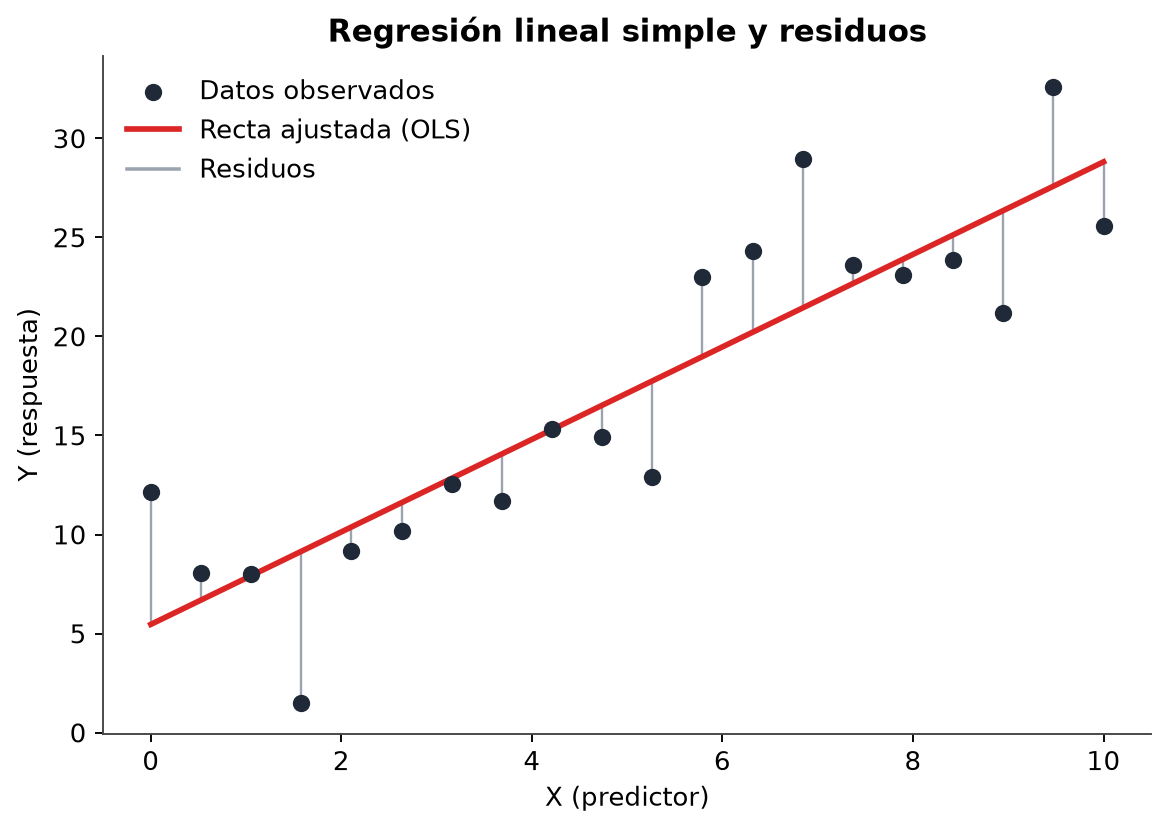
\includegraphics[width=0.4\textwidth]{../book/_static/generated/figures/es/linear_regression_fit.png}
  \end{center}
\end{frame}

\begin{frame}{Ejemplo real: dataset \textit{Advertising}}
  Un ejemplo clásico de la literatura es el conjunto de datos \textit{Advertising}, donde se ajusta una recta que predice las ventas (\texttt{Sales}) a partir de la inversión en publicidad en TV (\texttt{TV}). Cada punto gris vertical representa un \textbf{residuo}: la distancia entre el valor observado y el que predice la recta.
  \begin{center}
    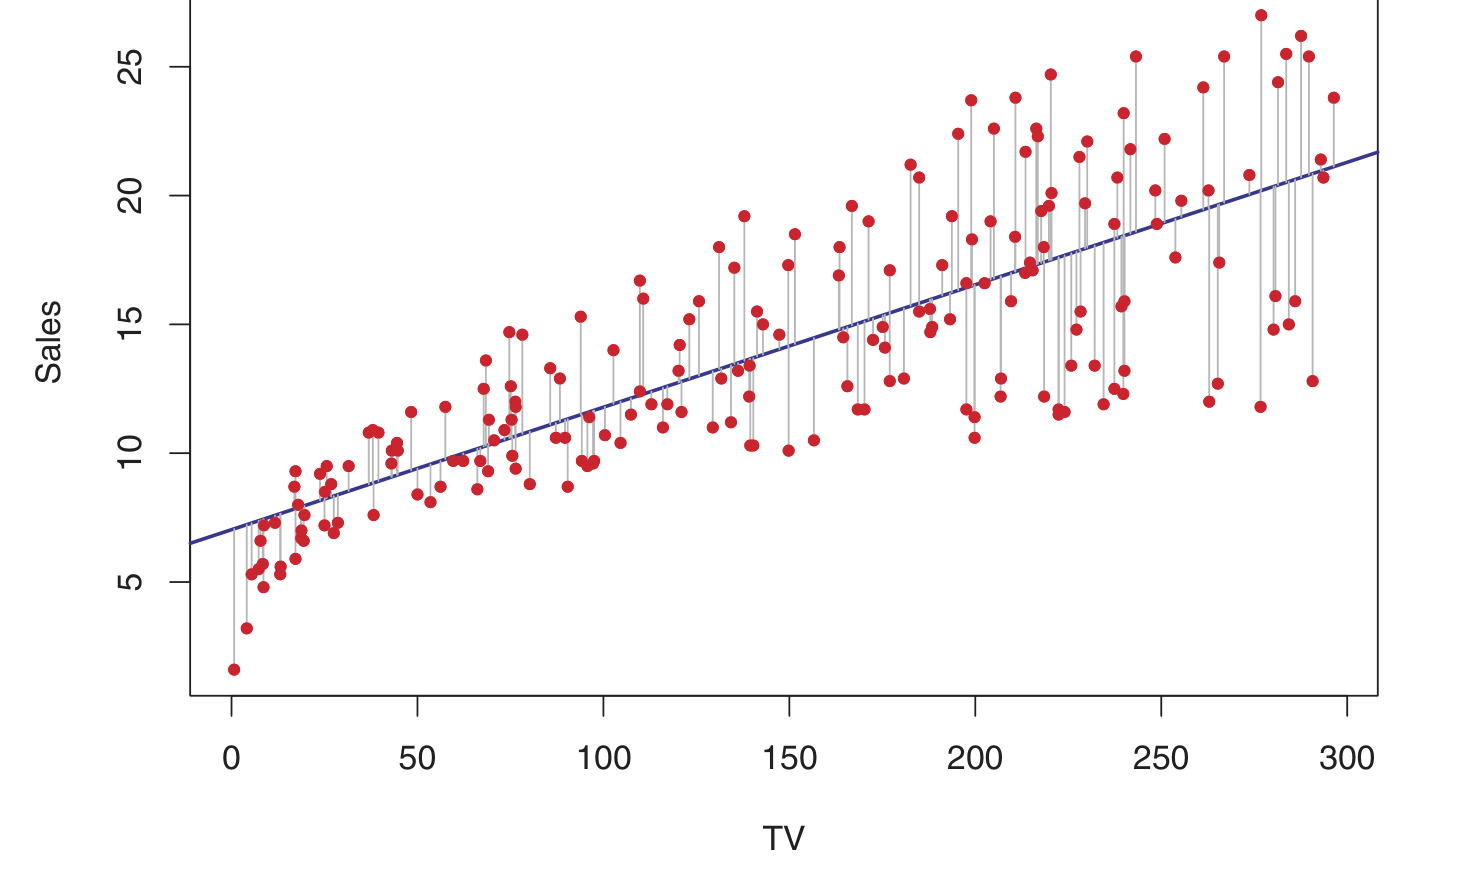
\includegraphics[width=0.42\textwidth]{../book/_static/book_figures/islr_fig3_1_advertising.png}
  \end{center}
  \fuente{James, Witten, Hastie \& Tibshirani (2013), \textit{An Introduction to Statistical Learning}, Fig. 3.1. Libro de libre distribución (statlearning.com).}
\end{frame}

\begin{frame}{Mínimos cuadrados ordinarios (OLS)}
  El método de \textbf{mínimos cuadrados ordinarios} (OLS) es el enfoque estándar para entrenar modelos lineales.
  \begin{itemize}
    \item Un \textbf{residual} $e_i = y_i - \hat{y}_i$ es la diferencia entre el valor real y el predicho.
    \item OLS busca los parámetros que hacen que esos residuales, elevados al cuadrado y sumados, sean lo más pequeños posible (a esta suma se le llama RSS).
    \item A diferencia de otros modelos, la regresión lineal tiene una \textbf{solución exacta}: existe una fórmula que calcula directamente los mejores parámetros en un único paso, sin necesidad de ensayo y error.
  \end{itemize}
  \ejemplo{con solo unas pocas casas (m\textsuperscript{2} y precio), OLS encuentra en un único cálculo la recta que mejor resume esa relación.}
\end{frame}

\begin{frame}{Descenso de gradiente}
  \small
  Para conjuntos de datos masivos o modelos con miles de parámetros, resolver la ecuación exacta de OLS es demasiado costoso. El \textbf{descenso de gradiente} es el algoritmo de optimización iterativo que impulsa gran parte del aprendizaje automático moderno.
  \begin{itemize}
    \item El algoritmo parte de pesos aleatorios y los va ajustando poco a poco, dando pequeños pasos en la dirección que más reduce el error.
    \item La \textbf{tasa de aprendizaje} determina el tamaño de cada paso: si es muy alta, el algoritmo puede ``pasarse'' y no llegar a converger; si es muy baja, el entrenamiento será lentísimo.
    \item Variantes: \textit{Batch} (usa todos los datos en cada paso), \textit{Stochastic} (SGD, una sola muestra por paso) y \textit{Mini-batch} (un grupo pequeño, el más usado en la práctica).
  \end{itemize}
  \ejemplo{\footnotesize es como bajar una montaña con niebla: en cada paso sientes la pendiente bajo tus pies y avanzas hacia donde más desciende, hasta llegar al valle.}
  \begin{center}
    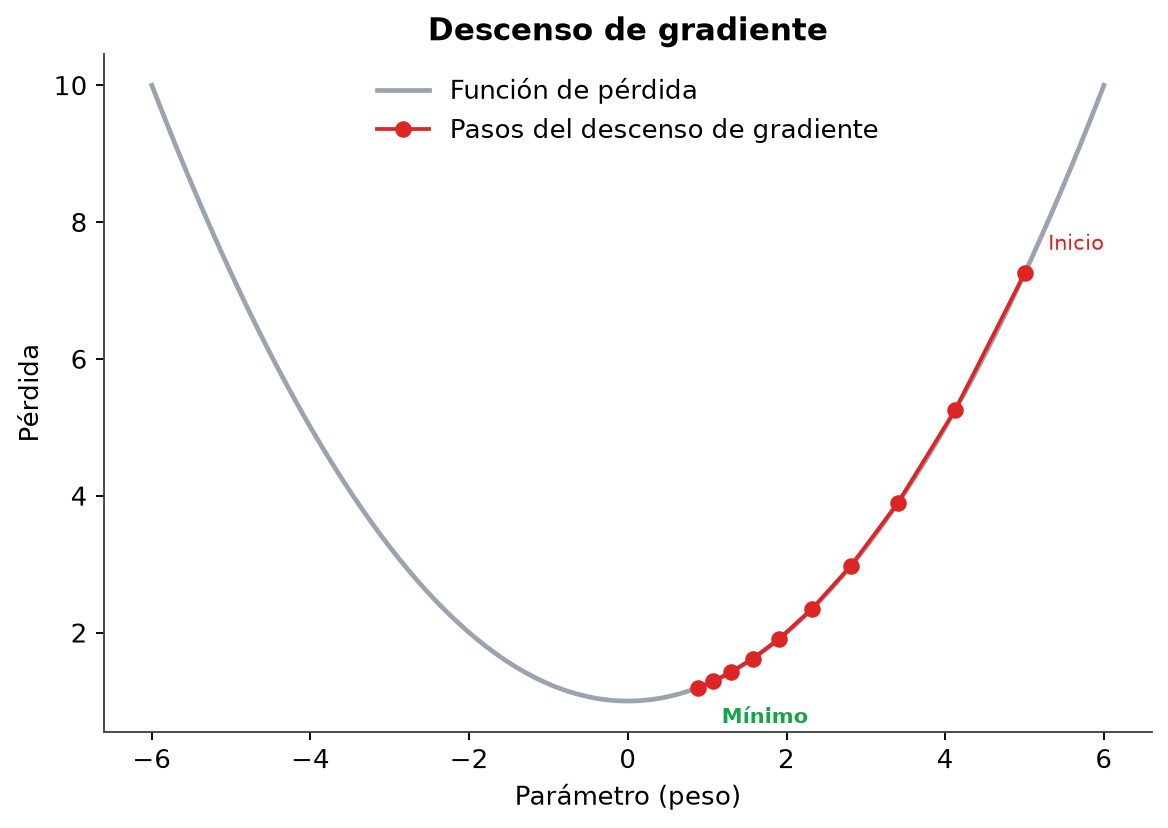
\includegraphics[width=0.19\textwidth]{../book/_static/generated/figures/es/gradient_descent.png}
  \end{center}
\end{frame}

\begin{frame}{Regresión polinomial}
  Cuando los datos presentan curvas, se pueden extender los modelos lineales mediante \textbf{ingeniería de características}: se añaden potencias de los predictores originales ($X^2$, $X^3$, \dots) como nuevas columnas de entrada.

  Aunque el modelo resultante es no lineal respecto a las variables originales, sigue siendo \textbf{lineal en sus parámetros}, así que se puede seguir entrenando con OLS o descenso de gradiente sin cambios.

  El riesgo: aumentar el grado del polinomio aumenta la flexibilidad del modelo, lo que puede llevarlo a memorizar el ruido de los datos de entrenamiento (\textit{overfitting}) en vez de captar la tendencia real.
\end{frame}

\begin{frame}{Regularización: \textit{Ridge} y \textit{Lasso}}
  Las técnicas de regularización añaden una penalización a la función de coste por tener pesos grandes, forzando al modelo a ser más simple y a generalizar mejor.
  \begin{itemize}
    \item \textbf{\textit{Ridge}}: encoge todos los coeficientes hacia cero, sin llegar nunca a eliminarlos; funciona muy bien cuando hay muchos predictores relacionados entre sí.
    \item \textbf{\textit{Lasso}}: penaliza de forma algo distinta y puede llevar algunos coeficientes exactamente a cero, haciendo así una \textbf{selección automática de variables}.
    \item \textbf{\textit{Elastic Net}}: combina ambas penalizaciones.
  \end{itemize}
  \begin{center}
    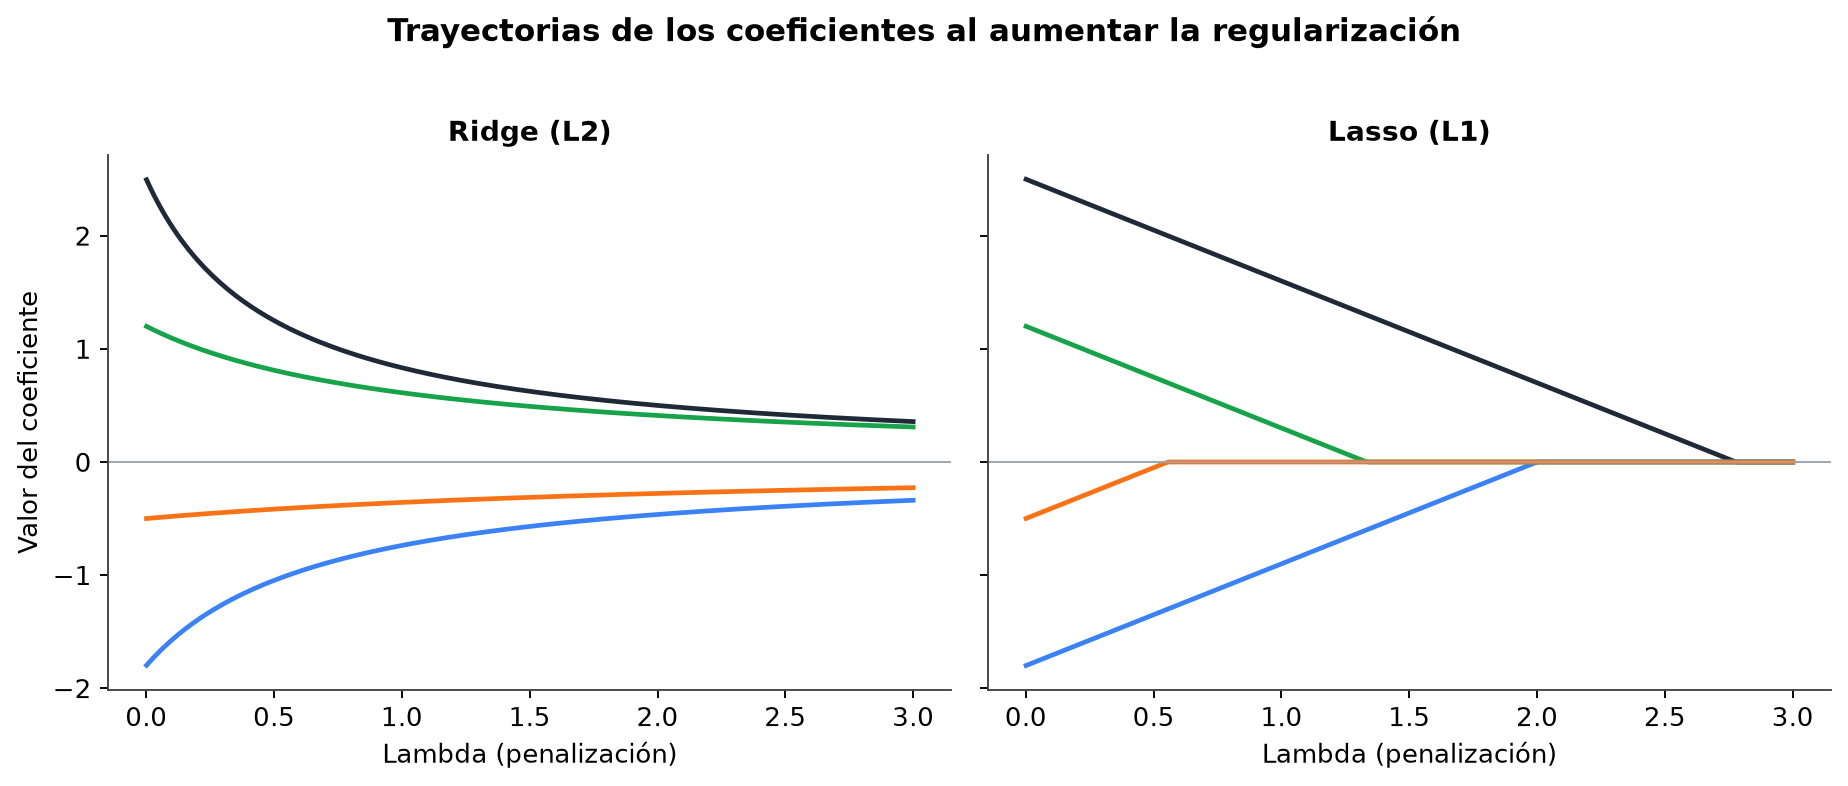
\includegraphics[width=0.5\textwidth]{../book/_static/generated/figures/es/regularization_paths.png}
  \end{center}
\end{frame}

\begin{frame}{Ridge en datos reales: dataset \textit{Credit}}
  Al aumentar el valor de $\lambda$ (la fuerza de la penalización), los coeficientes se encogen progresivamente hacia cero. Esto reduce la \textbf{varianza} del modelo a cambio de un pequeño aumento del \textbf{sesgo} --- exactamente el equilibrio que buscamos al regularizar.
  \begin{center}
    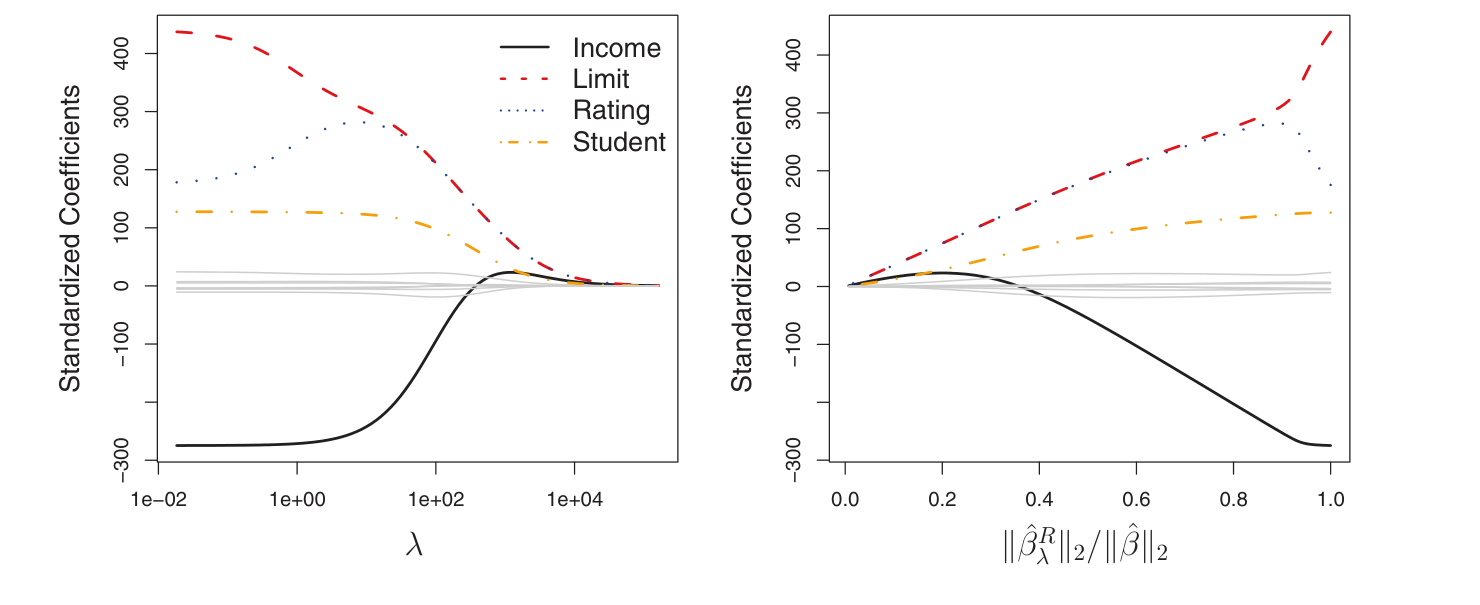
\includegraphics[width=0.5\textwidth]{../book/_static/book_figures/islr_fig6_4_ridge_credit.png}
  \end{center}
  \fuente{James, Witten, Hastie \& Tibshirani (2013), \textit{An Introduction to Statistical Learning}, Fig. 6.4.}
\end{frame}

\begin{frame}{Validación y diagnóstico en regresión}
  \small
  \begin{itemize}
    \item \textbf{MSE}/\textbf{RMSE}: penalizan fuertemente los errores grandes; el RMSE se expresa en las mismas unidades que $Y$, lo que facilita interpretarlo.
    \item \textbf{MAE} (error absoluto medio): el error medio ``típico'', más robusto ante valores atípicos que el MSE.
    \item \textbf{$R^2$}: qué proporción de la variación de $Y$ logra explicar el modelo. 1 = ajuste perfecto; 0 = tan bueno como predecir siempre la media.
    \item \textbf{Análisis de residuos}: si al graficar los errores del modelo aparece un patrón claro en vez de ruido aleatorio, es señal de que el modelo lineal se está quedando corto.
  \end{itemize}
\end{frame}

% ============================================================
\section{2.2 Clasificación}

\begin{frame}{Clasificación: predecir categorías}
  En clasificación, el objetivo es predecir una \textbf{categoría} (clase) en lugar de un valor continuo. Algunos ejemplos típicos: clasificación de correos (\textit{spam} vs. no \textit{spam}), clasificación médica (enfermo vs. sano) o clasificación de especies (gato vs. perro).

  A diferencia de la regresión lineal, la clasificación comienza estimando la \textbf{probabilidad} de que una muestra pertenezca a una categoría concreta.
\end{frame}

\begin{frame}{Regresión logística: la función sigmoide}
  \small
  La regresión logística utiliza la \textbf{función sigmoide} para convertir una combinación lineal de las características de entrada en una \textbf{probabilidad}, un valor siempre entre 0 y 1:
  \[ \sigma(t) = \frac{1}{1+e^{-t}} \]
  Cuanto mayor es $t$, más se acerca la salida a 1 (clase positiva); cuanto menor, más se acerca a 0.

  El modelo se entrena ajustando sus pesos, mediante descenso de gradiente, para que las probabilidades que predice se parezcan lo máximo posible a las etiquetas reales (0 o 1), penalizando con fuerza las predicciones que son seguras pero incorrectas.
  \begin{center}
    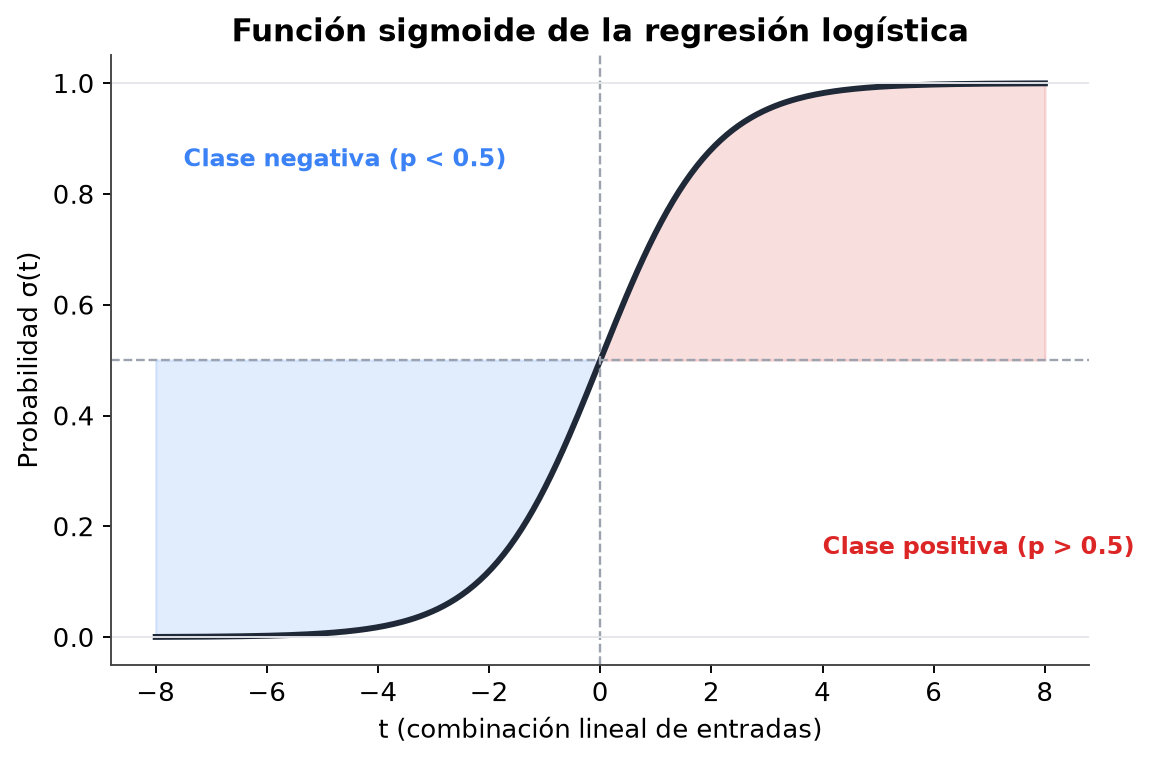
\includegraphics[width=0.34\textwidth]{../book/_static/generated/figures/es/sigmoid_function.png}
  \end{center}
\end{frame}

\begin{frame}{¿Por qué no usar regresión lineal?}
  La regresión lineal puede predecir probabilidades menores que 0 o mayores que 1, lo cual no tiene sentido. La regresión logística, gracias a la sigmoide, mantiene la salida siempre dentro del rango $[0,1]$.

  El siguiente ejemplo compara ambos ajustes sobre el conjunto de datos \textit{Default} (impago de crédito): a la izquierda, la regresión lineal produce probabilidades absurdas; a la derecha, la regresión logística siempre produce probabilidades válidas.
  \begin{center}
    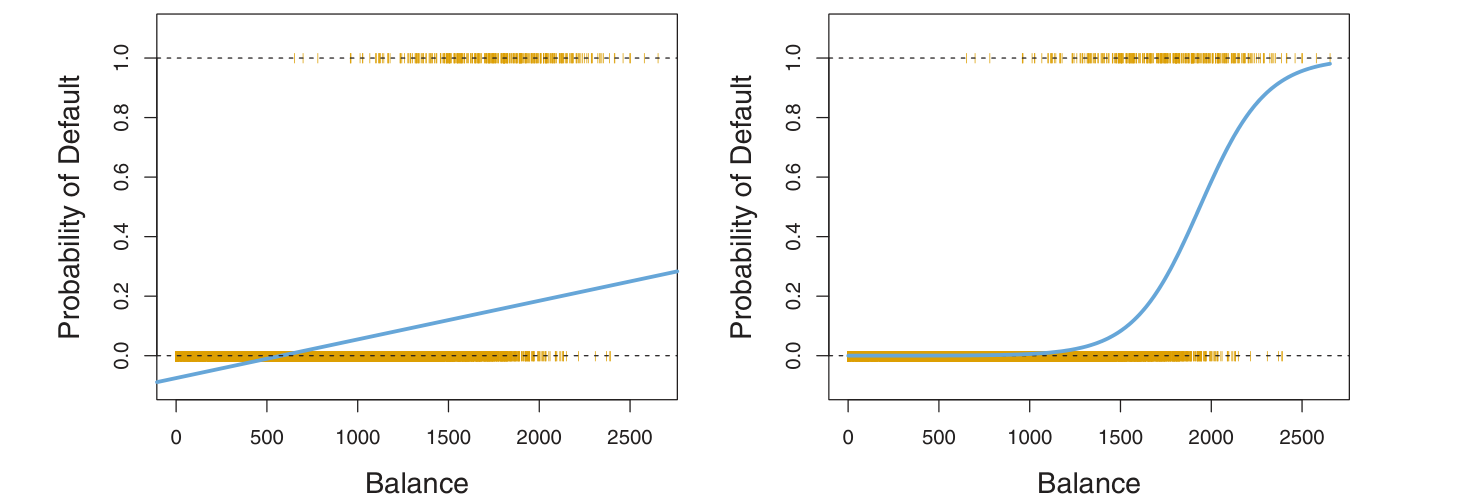
\includegraphics[width=0.55\textwidth]{../book/_static/book_figures/islr_fig4_2_default_logistic.png}
  \end{center}
  \fuente{James, Witten, Hastie \& Tibshirani (2013), \textit{An Introduction to Statistical Learning}, Fig. 4.2.}
\end{frame}

\begin{frame}{Árboles de decisión}
  \small
  Los árboles particionan el espacio de entrada de forma recursiva en ``cajas'' rectangulares, siguiendo un enfoque de ``divide y vencerás''.
  \begin{columns}
    \begin{column}{0.45\textwidth}
      \begin{itemize}
        \item \textbf{Construcción}: el árbol hace preguntas binarias sucesivas (``¿esta variable supera este valor?''), eligiendo en cada paso la que mejor separa las clases.
        \item \textbf{Poda} (\textit{pruning}): para evitar el sobreajuste, se eliminan ramas innecesarias basándose en pruebas estadísticas o en un conjunto de validación.
      \end{itemize}
    \end{column}
    \begin{column}{0.5\textwidth}
      \centering
      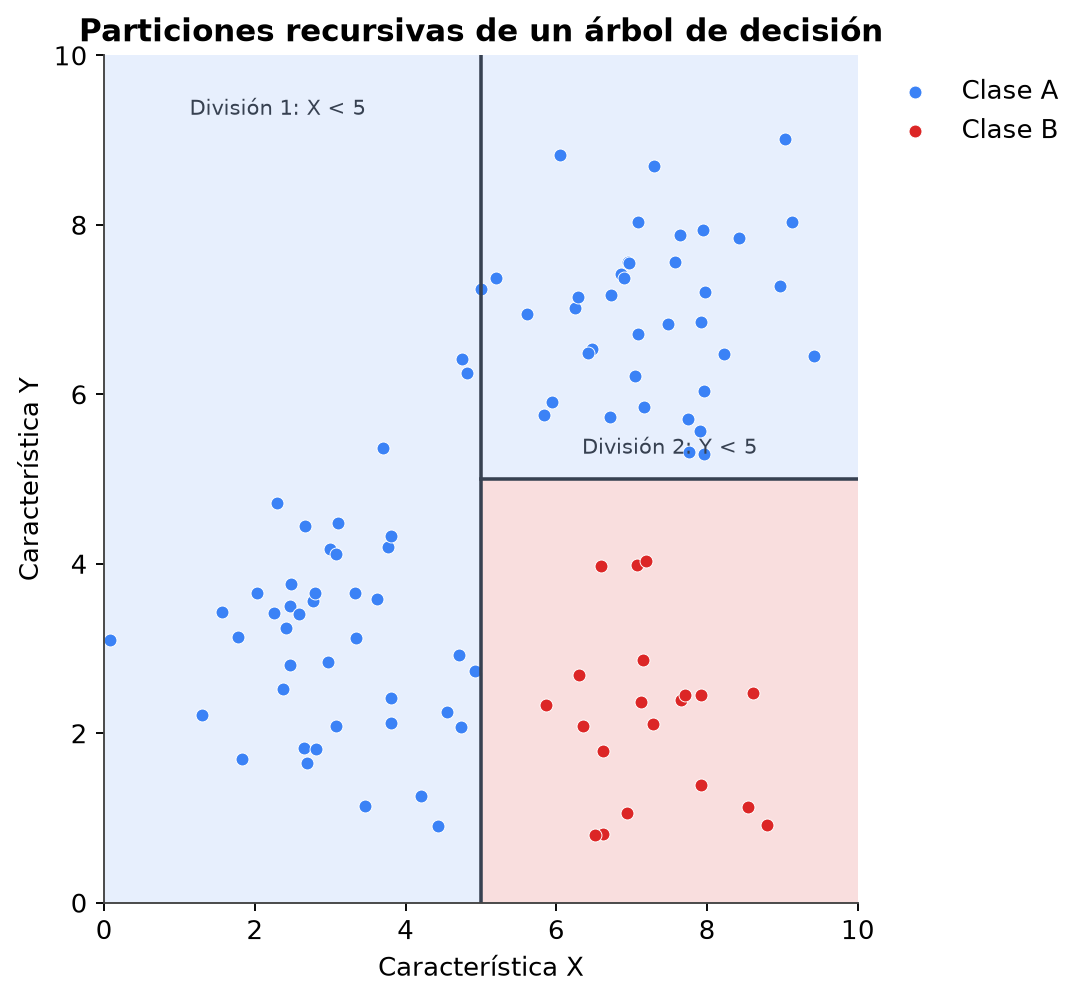
\includegraphics[width=0.82\textwidth]{../book/_static/generated/figures/es/decision_tree_partition.png}
    \end{column}
  \end{columns}
  \ejemplo{\footnotesize ``¿el email contiene la palabra `gratis'\,? $\rightarrow$ sí $\rightarrow$ ¿tiene más de 3 enlaces? $\rightarrow$ sí $\rightarrow$ \textit{spam}''.}
\end{frame}

\begin{frame}{Bosques aleatorios (\textit{Random Forests})}
  \small
  Un bosque aleatorio es un conjunto de muchos árboles de decisión, diseñado para reducir la varianza y mejorar la robustez frente a un único árbol.
  \begin{itemize}
    \item \textbf{\textit{Bagging}}: cada árbol se entrena con una muestra \textit{bootstrap} distinta (obtenida por muestreo con reemplazo del conjunto original).
    \item \textbf{Decorrelación}: en cada división solo se considera un subconjunto aleatorio de \textit{features}, para asegurar que los árboles sean diversos entre sí.
    \item Las predicciones individuales se combinan mediante \textbf{votación mayoritaria} (clasificación) o \textbf{promedio} (regresión).
  \end{itemize}
  \begin{center}
    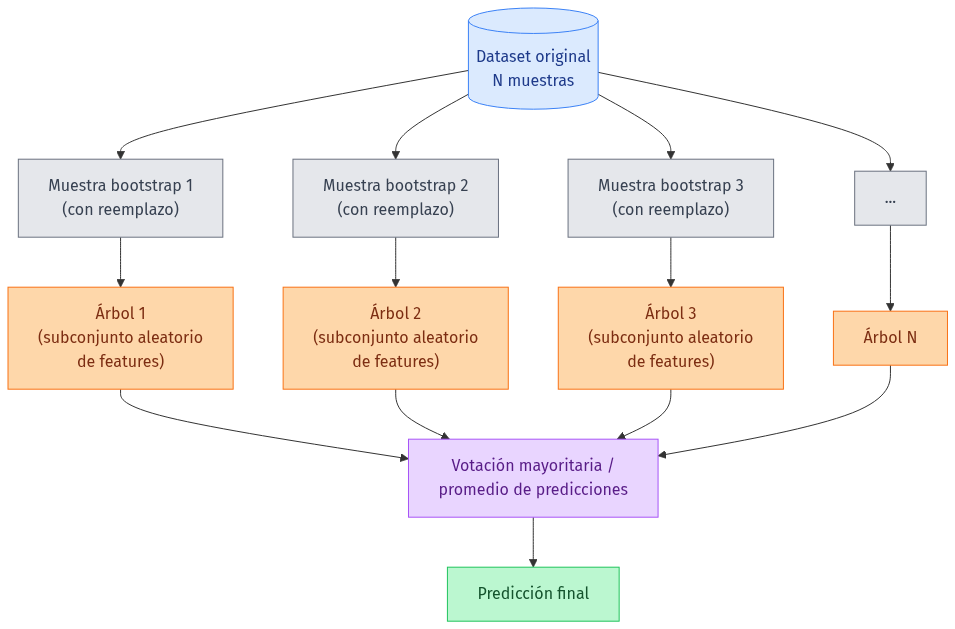
\includegraphics[width=0.34\textwidth]{../book/_static/generated/diagrams_pdf/es/01_aprendizaje_supervisado_02_clasificacion_01.png}
  \end{center}
\end{frame}

\begin{frame}{Máquinas de vectores de soporte (SVM)}
  \begin{columns}
    \begin{column}{0.45\textwidth}
      Este modelo busca el \textbf{hiperplano} que separa las clases con el \textbf{margen máximo} posible.
      \begin{itemize}
        \item Los \textbf{vectores de soporte} son las únicas muestras que determinan la posición de la frontera; mover cualquier otro punto no altera el modelo.
        \item Con datos no separables linealmente, el \textbf{margen blando} permite algunos errores, y el \textbf{truco del \textit{kernel}} mapea implícitamente los datos a un espacio de más dimensiones donde sí son separables.
      \end{itemize}
    \end{column}
    \begin{column}{0.5\textwidth}
      \centering
      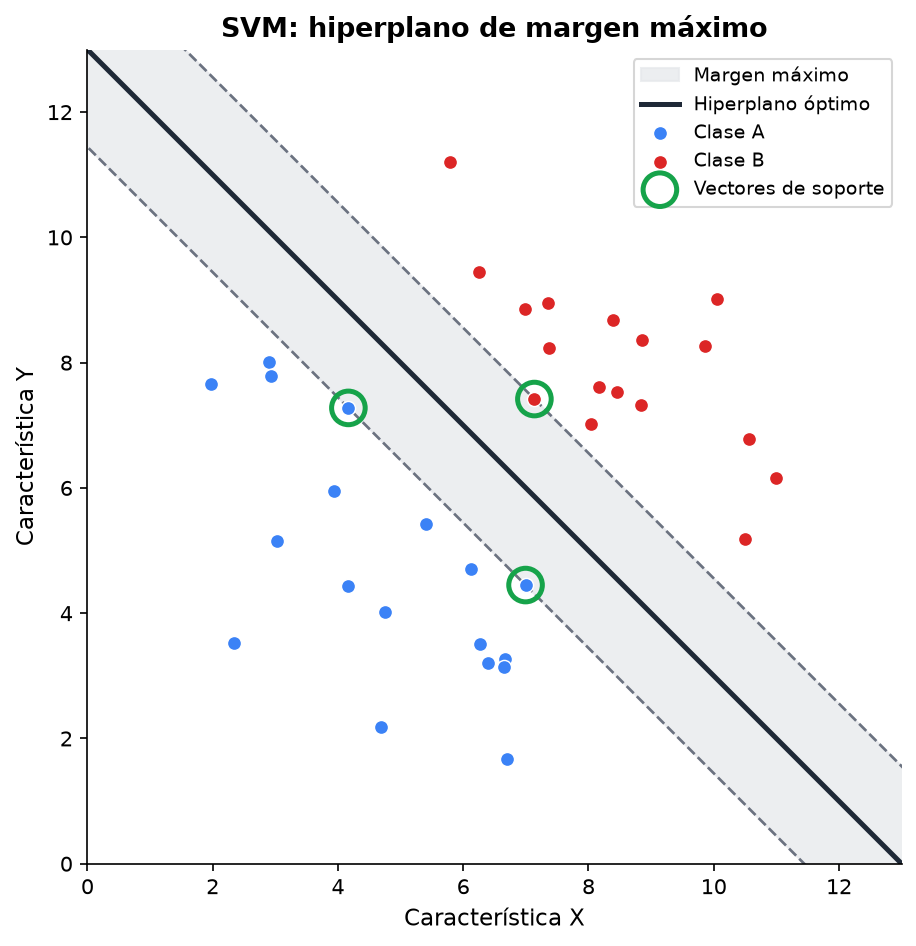
\includegraphics[width=\textwidth]{../book/_static/generated/figures/es/svm_margin.png}
    \end{column}
  \end{columns}
\end{frame}

\begin{frame}{\textit{Voting} y \textit{stacking}}
  \small
  Los métodos de ensamble combinan varios modelos para obtener una predicción superior a la de cualquiera de ellos por separado.
  \begin{itemize}
    \item \textbf{\textit{Voting}}: combina modelos independientes mediante una regla fija --- voto mayoritario (``duro'') o promedio de probabilidades (``suave'').
    \item \textbf{\textit{Stacking}}: entrena un \textbf{meta-modelo} que aprende, a partir de datos, cómo combinar las salidas de los modelos base --- una regla aprendida, no fija.
  \end{itemize}
  \begin{center}
    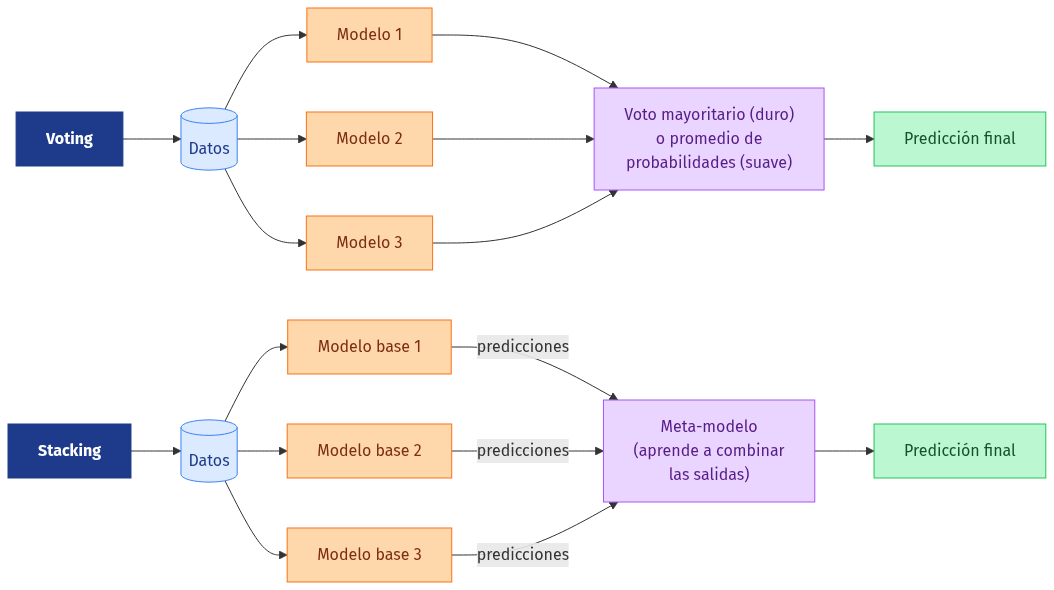
\includegraphics[width=0.5\textwidth]{../book/_static/generated/diagrams_pdf/es/01_aprendizaje_supervisado_02_clasificacion_03.png}
  \end{center}
\end{frame}

\begin{frame}{\textit{Boosting}}
  A diferencia del entrenamiento en paralelo de los bosques aleatorios, el \textit{boosting} entrena modelos de forma \textbf{secuencial}: cada nuevo modelo se centra en corregir los errores cometidos por el anterior, dando más peso a las instancias mal clasificadas. La predicción final combina todos los modelos mediante una suma ponderada.

  Ejemplos modernos y muy usados en competiciones de datos: \textbf{XGBoost} y \textbf{\textit{Gradient Boosting}}.
  \begin{center}
    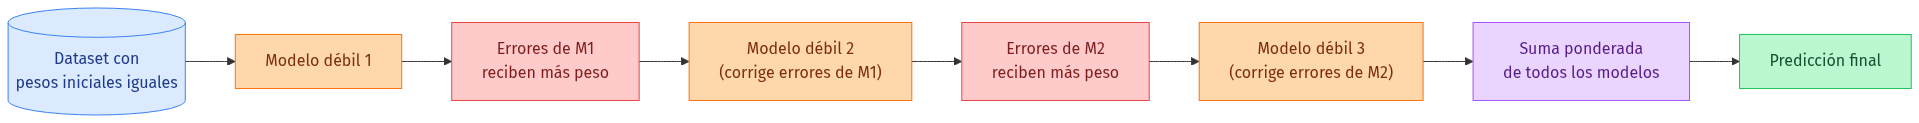
\includegraphics[width=0.78\textwidth]{../book/_static/generated/diagrams_pdf/es/01_aprendizaje_supervisado_02_clasificacion_02.png}
  \end{center}
\end{frame}

\begin{frame}{Redes neuronales}
  \small
  Las redes neuronales representan el aprendizaje de representaciones sucesivas a través de capas de filtrado.
  \begin{itemize}
    \item \textbf{Arquitectura}: una capa de entrada, una o varias capas ocultas (densamente conectadas) y una capa de salida.
    \item \textbf{Funciones de activación}: introducen no linealidad para poder aprender patrones complejos. \textbf{ReLU} es el estándar en capas ocultas; \textbf{Softmax} se usa en la capa de salida para clasificación de múltiples clases.
    \item \textbf{Retropropagación} (\textit{backpropagation}): el mecanismo central de aprendizaje. Propaga el error desde la salida hacia atrás, capa por capa, ajustando los pesos de la red para reducir la pérdida total.
  \end{itemize}
  \begin{center}
    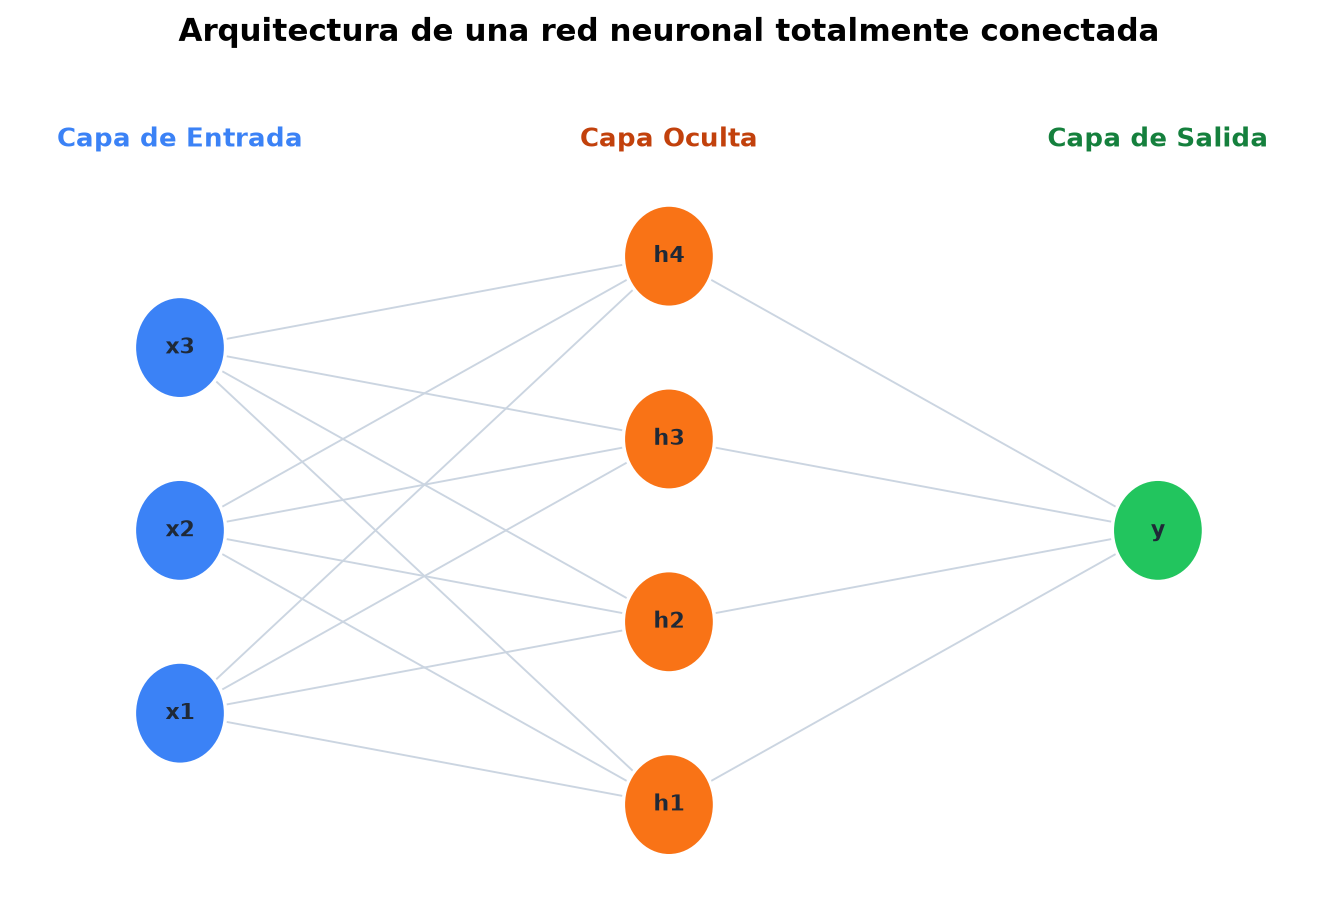
\includegraphics[width=0.24\textwidth]{../book/_static/generated/figures/es/nn_architecture.png}
  \end{center}
\end{frame}

\begin{frame}{Evaluación: protocolos de validación}
  \small
  Igual que en regresión, es obligatorio dividir los datos en particiones independientes para medir bien la generalización:
  \begin{itemize}
    \item \textbf{Entrenamiento}, \textbf{validación} y \textbf{prueba}: un conjunto para ajustar pesos, otro para elegir hiperparámetros y un tercero, intacto, para la evaluación final.
    \item \textbf{Validación cruzada de $K$ pliegues}: la estrategia recomendada cuando los datos son escasos.
    \item \textbf{Estratificación}: en clasificación, cada partición debe mantener la proporción original de clases, sobre todo si están desbalanceadas.
  \end{itemize}
\end{frame}

\begin{frame}{Evaluación: métricas de éxito}
  \small
  Las mismas métricas vistas en el capítulo anterior (exactitud, precisión, \textit{recall}, F1, ROC-AUC) se aplican aquí, y son igual de importantes:
  \begin{itemize}
    \item \textbf{Exactitud} puede ser engañosa en datos desbalanceados: si el 90\% de las muestras son de una clase, predecir siempre esa clase da 90\% de exactitud sin haber aprendido nada.
    \item Por eso conviene mirar también \textbf{precisión} y \textbf{\textit{recall}}, sobre todo cuando el coste de un error depende de qué clase se confunde.
  \end{itemize}
  \begin{center}
    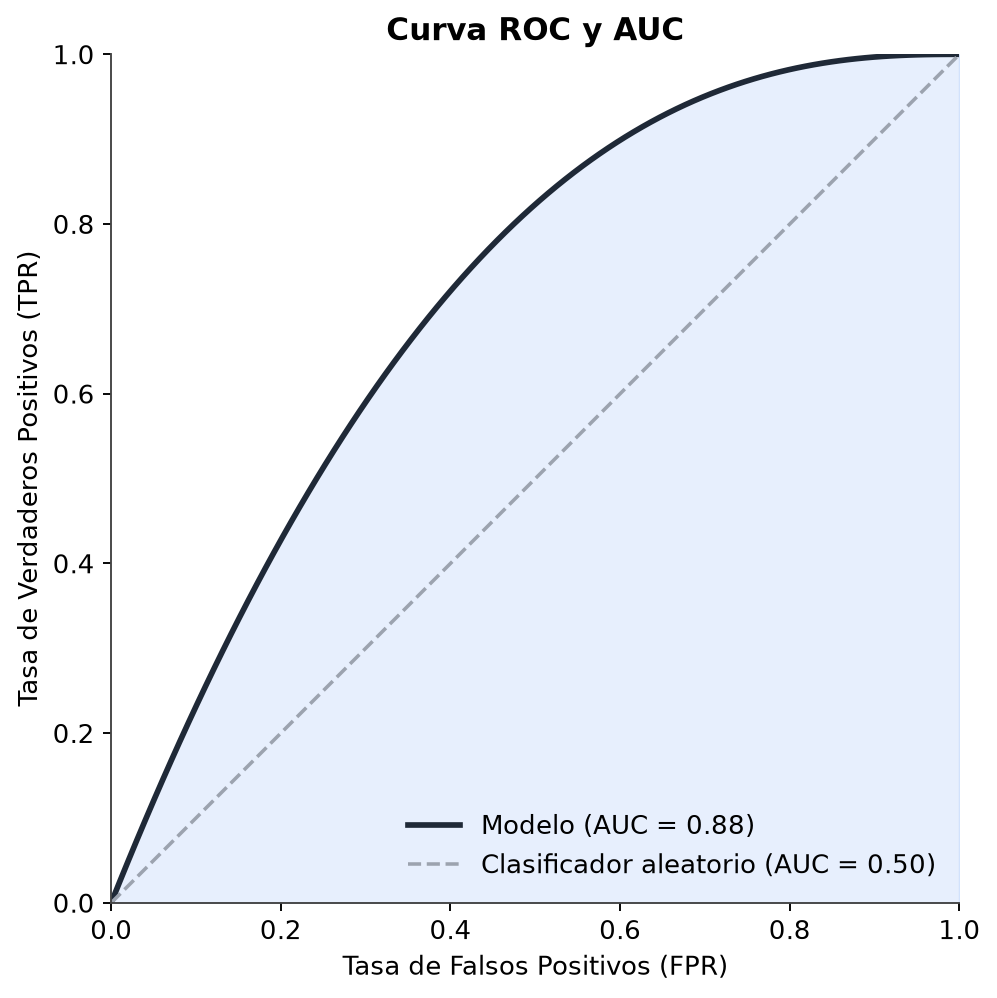
\includegraphics[width=0.22\textwidth]{../book/_static/generated/figures/es/roc_curve.png}
  \end{center}
\end{frame}

\begin{frame}{Estrategias de entrenamiento y diagnóstico}
  \small
  La evaluación no ocurre solo al final: debe guiar todo el proceso de desarrollo.
  \begin{itemize}
    \item \textbf{Superar una línea de base}: antes de complicarse con modelos avanzados, hay que comprobar que se supera algo muy simple (por ejemplo, predecir siempre la clase más común).
    \item \textbf{Curvas de aprendizaje}: graficar el error de entrenamiento y validación a lo largo del entrenamiento revela el punto exacto en que aparece el sobreajuste.
    \item \textbf{Parada temprana} (\textit{early stopping}): interrumpe el entrenamiento automáticamente cuando el modelo deja de mejorar en validación.
    \item \textbf{Análisis de errores}: revisar a mano los casos donde falla el modelo ayuda a entender qué lo está confundiendo.
  \end{itemize}
\end{frame}

% ============================================================
\begin{frame}{Resumen del capítulo}
  \small
  \begin{itemize}
    \item En \textbf{regresión} predecimos un valor continuo; en \textbf{clasificación}, una categoría.
    \item \textbf{OLS} da una solución exacta; el \textbf{descenso de gradiente} escala a datos masivos.
    \item La \textbf{regularización} (\textit{Ridge}/\textit{Lasso}) evita el sobreajuste penalizando los pesos grandes.
    \item La \textbf{regresión logística} extiende la idea de la regresión lineal a probabilidades mediante la sigmoide.
    \item \textbf{Árboles}, \textbf{\textit{Random Forest}} y \textbf{SVM} son alternativas clásicas de clasificación, cada una con sus ventajas.
    \item Los métodos de \textbf{ensamble} (\textit{voting}, \textit{stacking}, \textit{boosting}) combinan modelos para mejorar el resultado.
    \item Las \textbf{redes neuronales} aprenden representaciones en capas mediante retropropagación.
    \item Evaluar bien --- con las particiones y métricas adecuadas --- es tan importante como entrenar bien.
  \end{itemize}
\end{frame}

% ============================================================
\begin{frame}{Licencia de estas diapositivas}
  \begin{center}
    Este material se distribuye bajo licencia\\[0.3em]
    {\large\textbf{\textcolor{usalred}{Creative Commons Reconocimiento-NoComercial 4.0}}}\\[0.2em]
    {\footnotesize (CC BY-NC 4.0)}
  \end{center}
  \vspace{0.3em}
  \small
  \begin{columns}[t]
    \begin{column}{0.47\textwidth}
      \textbf{\textcolor{usalred}{Eres libre de:}}
      \begin{itemize}
        \item \textbf{Compartir}: copiar y redistribuir el material en cualquier medio o formato.
        \item \textbf{Adaptar}: remezclar, transformar y crear a partir del material.
      \end{itemize}
      {\footnotesize Por ejemplo: usarlas en clase, subirlas al aula virtual, traducirlas o reutilizar una figura en tus apuntes.}
    \end{column}
    \begin{column}{0.47\textwidth}
      \textbf{\textcolor{usalred}{Con estas condiciones:}}
      \begin{itemize}
        \item \textbf{Reconocimiento (BY)}: debes citar la autoría, enlazar a la licencia e indicar si has hecho cambios.
        \item \textbf{NoComercial (NC)}: no puedes usar el material con fines comerciales.
      \end{itemize}
      {\footnotesize No puedes añadir restricciones que impidan a otros hacer lo que la licencia permite.}
    \end{column}
  \end{columns}
  \vspace{0.4em}
  \begin{center}
    {\footnotesize\texttt{creativecommons.org/licenses/by-nc/4.0/deed.es}}
  \end{center}
\end{frame}

\titleslide

\end{document}
